\chapter{Závěr}

\section{Současný stav aplikace}
Nástroj MT-ComparEval je v~současné době plně funkční.
Umožňuje spravovat experimenty a jejich tasky.
Tasky je možné porovnávat na základě různých kriterií -
  hodnot metrik strojového překladu,
  porovnání jednotlivých vět
  či přehledu nejvíce zlepšujících a zhoršujících \mbox{n-gramů}.
Při porovnání překladů jedné věty je možné si nechat zvýraznit
  potvrzené \mbox{n-gramy}, zlepšující \mbox{n-gramy}, zhoršující \mbox{n-gramy}, diff mezi překlady
  či jeden z~nejvíce zlepšujících nebo zhoršujících \mbox{n-gramů}.


\section{Nápady na vylepšení}
I~přes to, že nástroj MT-ComparEval umožňuje porovnávat dvě různé verze překladů,
  existuje mnoho způsobů,
  jak by tento nástroj šlo vylepšit.

\subsection{Podpora více referencí}
Při vyhodnocování strojových překladů a počítání metrik používá nástroj MT-ComparEval pouze porovnání s~jednou referencí.
Protože většina vět může být přeložena různými způsoby,
  může nastat situace,
  kdy daný překlad neodpovídá zvolené referenci.
Aby bylo možné takové překlady lépe ohodnotit,
  mohly by být překlady porovnávány s~několika různými referencemi.
Z~těchto referencí by pak byla vybrána ta,
  pro kterou by daný překlad dosáhl nejlepšího skóre.
Z~tohoto důvodu by bylo dalším možným rozšířením přidání podpory více referencí v~experimentu.

\subsection{Více metrik}
I~přes to, že metrika BLEU silně odpovídá lidskému hodnocení překladů,
  nemusí být vždy považována za nejvhodnější pro jejich vyhodnocování.
Některé strojové překladače jsou speciálně optimalizovány na metriku BLEU,
  což ale v~konečném výsledku nemusí dávat zcela vhodné překlady.
Proto by bylo dalším vhodným rozšířením,
  vyhodnocování strojových překladačů na základě několika metrik.
Mezi metriky,
  které by bylo možné a vhodné do nástroje MT-ComparEval doprogramovat,
  patří např. NIST, METEOR, PORT,~\dots

\subsection{Zobrazení alignmentu}
Při porovnávání dvou překladů jedné věty je velmi užitečná funkce pro zvýraznění slov (nazývaná alignment),
  které odpovídají danému slovu v~referenci či dalším strojovém překladu.
Díky této funkci je pak snadnější analyzovat chovaní strojových překladačů.

Na Obrázku \ref{img:alignment} je ukázáno, jak zvýrazňuje aligment překladač Google Translate.
\begin{figure}
	\center
	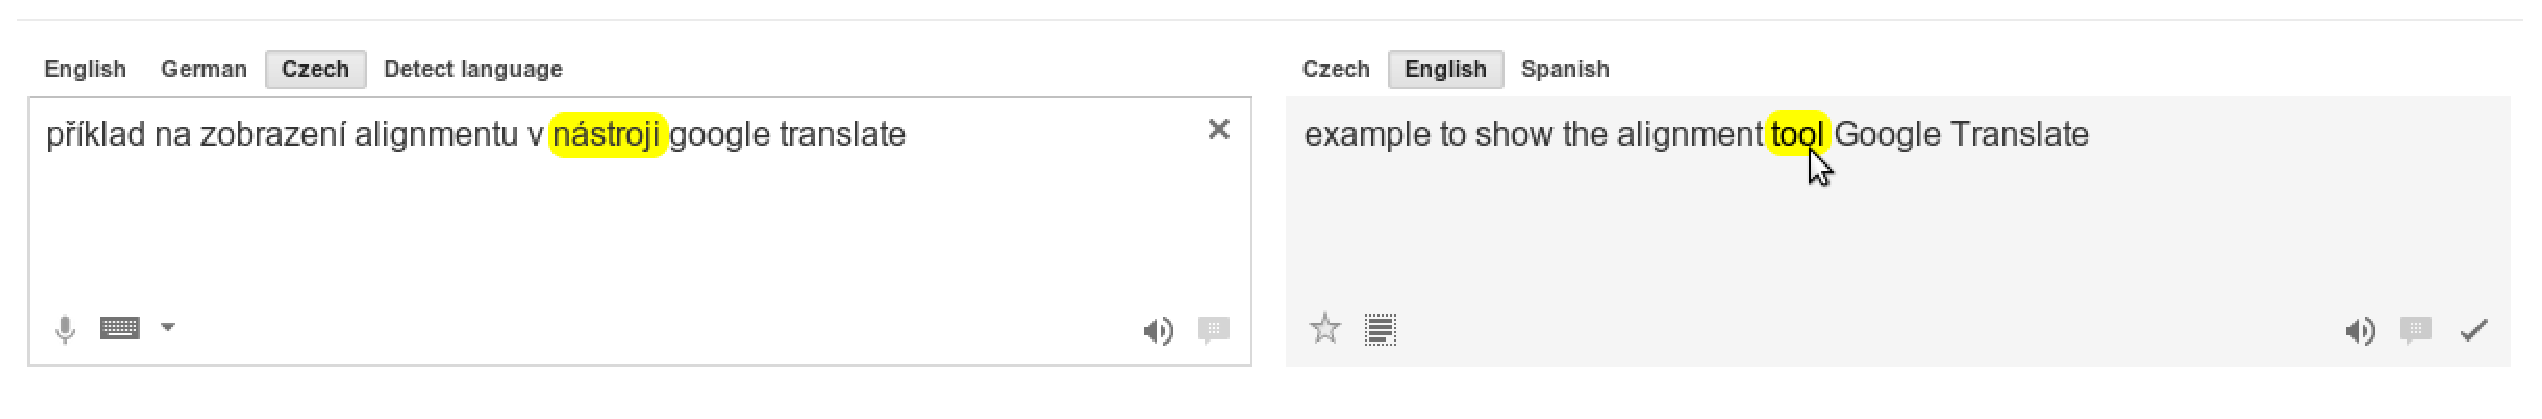
\includegraphics[width=0.9\textwidth]{img/alignment.eps}
	\caption{Ukázka zobrazení aligmentu v~překladači Google Translate}
	\label{img:alignment}
\end{figure}

\section{Podobné aplikace}
Vývoj nástroje MT-ComparEval byl v~určitých oblastech inspirován nástroji,
  které už jsou volně dostupné.
Z~těchto nástrojů byly vybrány nejdůležitější vlastnosti,
  které byly sloučeny do jednoho funkčního celku.
V~následující části budou tyto nástroje podrobněji představeny.

\subsection{mteval-11b.pl}
Je skript napsaný v~jazyce Perl,
  který umožňuje počítat metriky BLEU a NIST.
Tento skript je celosvětově používaný,
  a proto byl použit pro kontrolu,
  že je metrika BLEU v~MT-ComparEval počítána správně.

V~současné době už existuje verze mteval-13a.pl,
  v~které mimo jiné přibyla možnost počítat metriky pro jednotlivé segmenty v~překladu.

\subsection{iBLEU}
Nástroj iBLEU umožňuje vyhodnocovat a porovnávat strojové překlady.
Pokud uživatel nemá žadný jiný strojový překlad,
  se kterým by chtěl svůj překlad porovnat,
  může si větu nechat přeložit překladačem Google Translate\footnote{
    Bohužel Google Translate nenabízí bezplatné api.
  } nebo Bing Translator\footnote{
    Bing Translator nabízí bezplatné api do limitu 2 miliónů přeložených znaků za den.
  }
  a porovnat svůj překlad s~překladem z~těchto nástrojů.

Pomocí tohoto nástroje můžeme počítat BLEU pro celé dokumenty nebo i jednotlivé segmenty.
Je také možné si jednotlivé segmenty na základě těchto výsledků prohléhnout.

Pokud uživatel porovnává svůj překlad pouze s~referencí,
  je zvýrazněn jejich diff.
V~případě, že uživatel porovnává dva strojové překlady,
  je zobrazen diff těchto překladů.

Tento nástroj je možné používat lokálně jako webovou aplikaci bez použití webového serveru,
  protože je celý napsán v~HTML 5, CSS a javascriptu.
Stejně jako MT-ComparEval i iBLEU používá pro počítání BLEU jako referenční implementaci mteval-13a.pl.

Na Obrázku \ref{img:ibleu} je možné vidět porování dvou překladů v~nástroji iBLEU.
\begin{figure}
  \center
  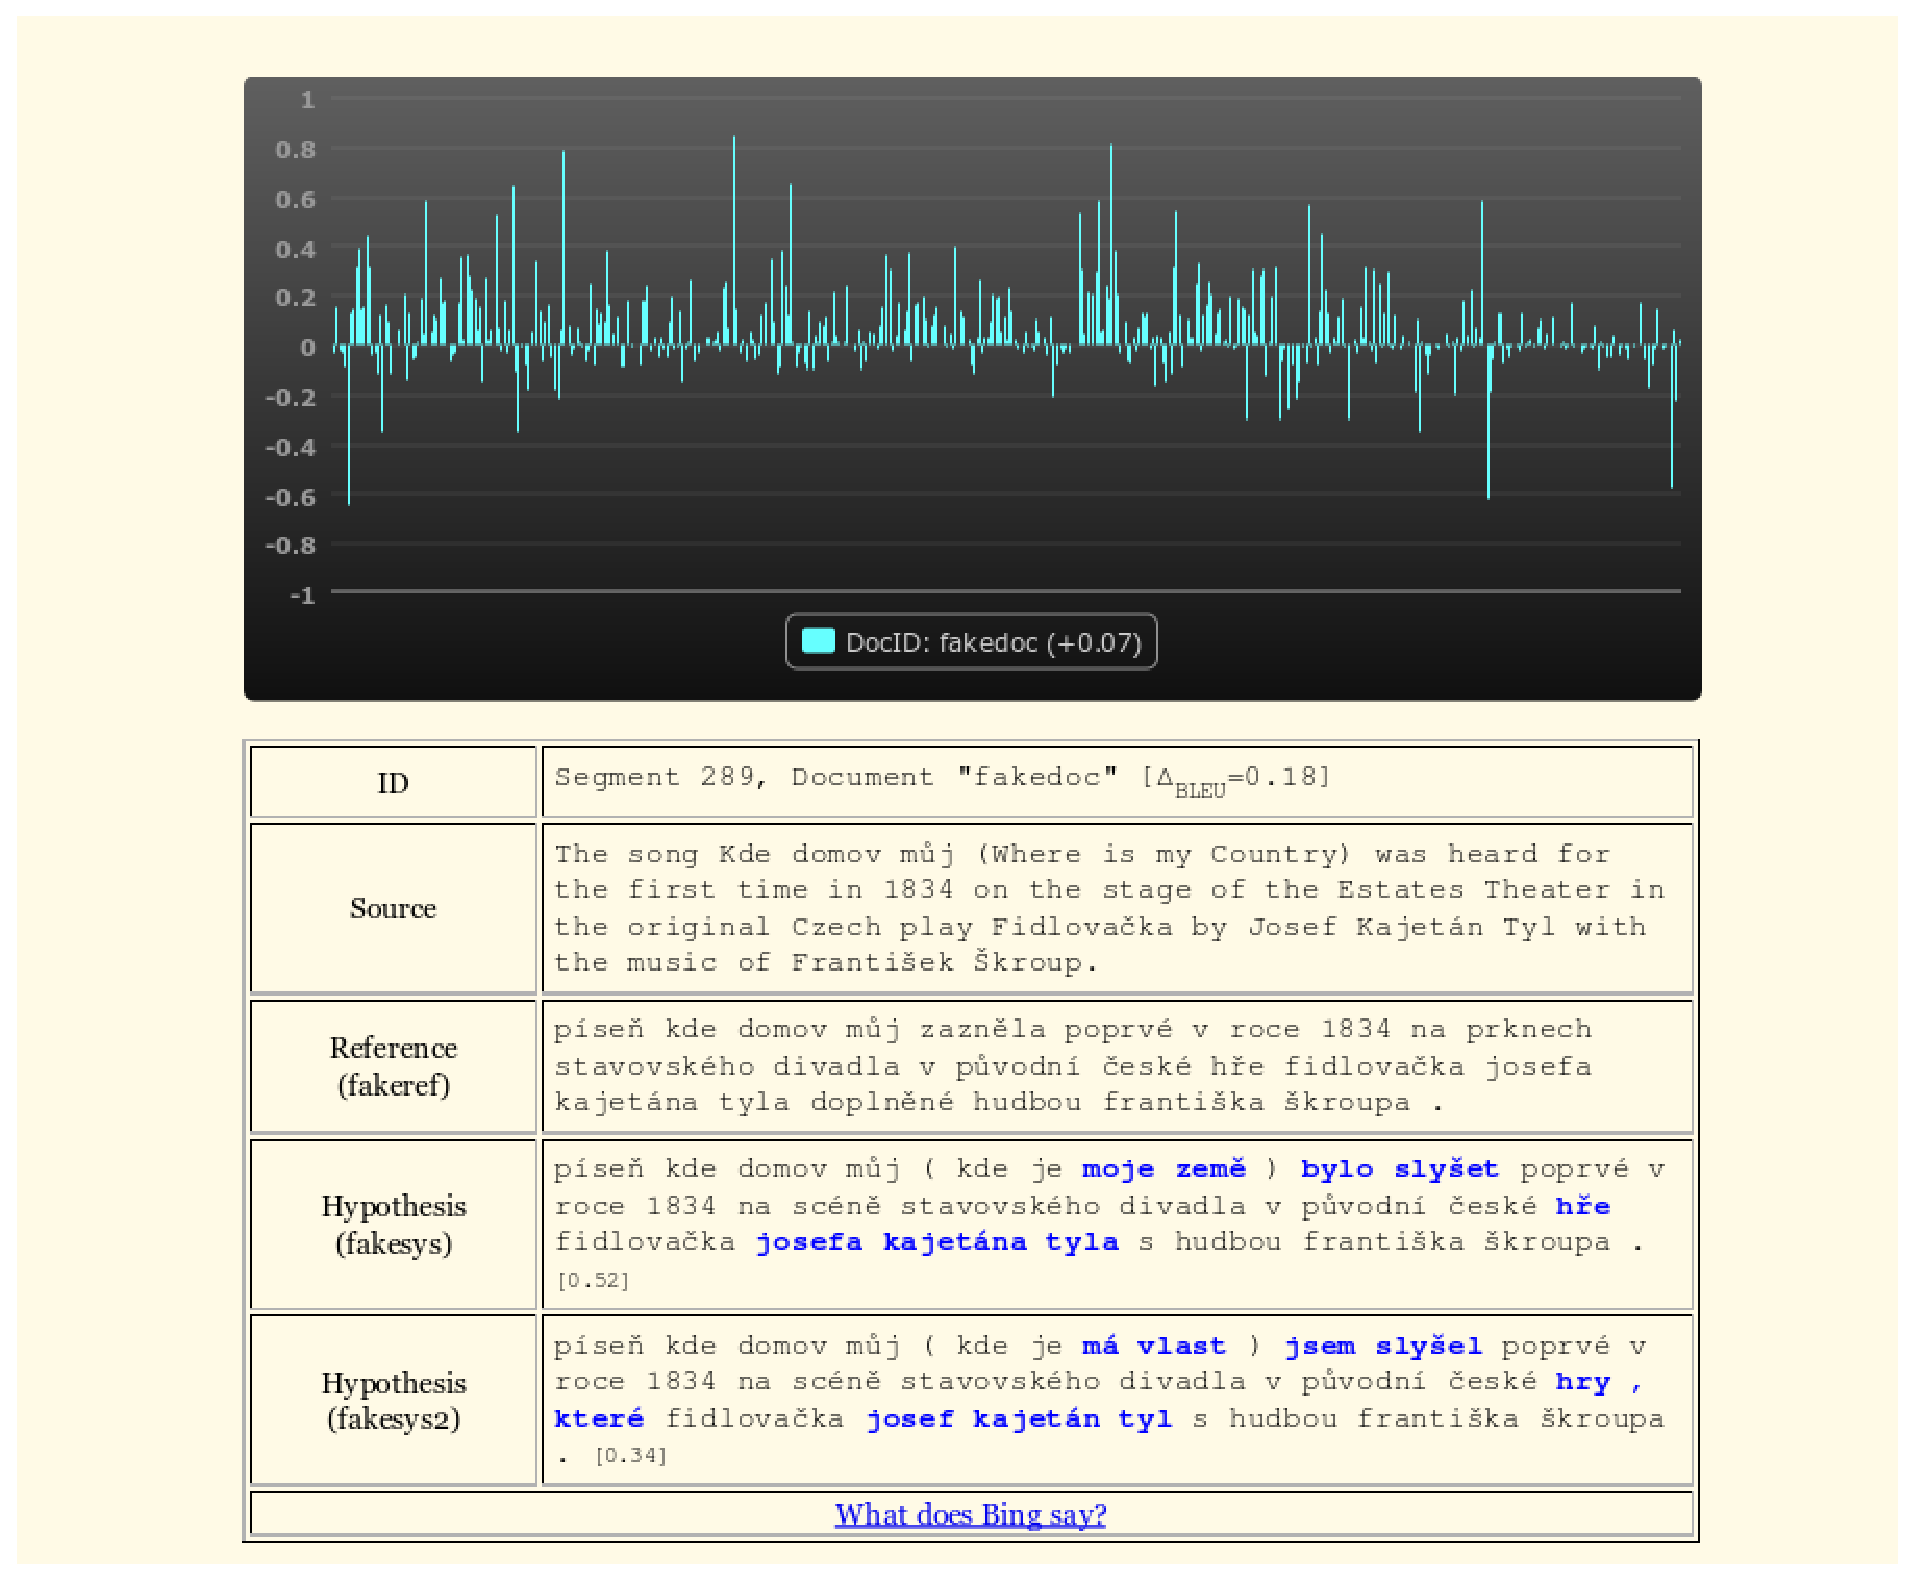
\includegraphics[width=0.9\textwidth]{img/ibleu.eps}
  \caption{Porovnání dvou překladů v~nástroji iBLEU}
  \label{img:ibleu}
\end{figure}


\subsection{EMS -- An Experimental Management System}
Nástroj EMS,
  který je součástí strojového překladače Moses,
  obsahuje webovou aplikaci,
  díky níž je možné porovnávat překlady.
V~porovnávaných větách barevně zvýrazňuje slova,
  na základě délky nejdelšího \mbox{n-gramu},
  do kterého zvýrazňované slovo patří.
Obrázek \ref{img:ems-sentence} ukazuje takto zvýrazněnou větu.
Pro \mbox{n-gramy} také počítá precision a recall.

\begin{figure}
  \caption{Zvýrazněné \mbox{n-gramy} podle délky v~nástroji EMS}
  \label{img:ems-sentence}
\end{figure}

Ve webovém prostředí je také možné vyhledávat věty,
  ve kterých byl použit \mbox{n-gram}.
Jednotlivá užití \mbox{n-gramů} jsou pak rozřazena do skupin podle správnosti překladu.
Na Obrázku \ref{img:ems-word} je možné vidět seznam vět,
  ve kterých bylo použito slovo ??.

\begin{figure}
  \caption{Výpis vět, ve kterých se vyskytuje slovo ??, v~nástroji EMS}
  \label{img:ems-word}
\end{figure}

Další věcí, kterou můžeme použít při porovnávání dvou překladů,
  jsou grafy správně přeložených vs. špatně přeložených slov.
Takové grafy je možné vidět na Obrázku \ref{img:ems-charts}.

\begin{figure}
  \caption{Grafy správně přeložených vs. špatně přeložených slov v~nástroji EMS}
  \label{img:ems-charts}
\end{figure}

Webové prostředí nástroje EMS nabízí i další možnosti porovnání překladů,
  o~kterých je možné se více dozvědět v~dokumentaci tohoto nástroje.

\section{Problémy při řešení}
Při vývoji nástroje MT-ComparEval jsem narazil na mnoho problémů.
Ať už se jednalo o~volbu jazyka, frameworku či databáze.

Aby bylo možné snadno nainstalovat nástroj MT-ComparEval na vybraném počítači,
  byla jako databáze zvolena databáze SQLite 3.
Ta vyhovuje většině požadavků.
Bohužel bylo hodně času věnováno odhalování chyb,
  způsobených tím,
  že SQLite 3 zamyká zvláštním způsobem datový soubor,
  a proto není možné používat databázi v~dalších procesech.
Při normálním použití na webu se s~touto chybou nepotkáme,
  protože procesy databázi používají pouze během zpracování HTTP požadavku.
Avšak při použití dlouho trvajících procesů pro import experimentů a tasků
  vždy docházelo ke kolizím při přístupu k~databázi,
  které vyústily v~pád importu.
Proto musel být návrh importu zcela přepracován a nyní by měl fungovat podle představ.
Nyní už import funguje správně a neměl by při něm nastat výše zmíněný problém.


V~duchu TDD\footnote{Test-Driven-Development}
  jsem se snažil před vlastní implementací napsat testy pomocí nástroje Behat.\footnote{http://www.behat.org}
Ten slouží k~BDD\footnote{Behaviour-Driven-Development}.
Pro všechny kroky importů byly napsány specifikace chování, které byly nástrojem Behat otestovány.
Ovšem později se ukázalo, že tento přístup k~testování nebyl úplně vhodný, a testy pomocí tohoto nástroje jsem přestal psát.
Vše bylo způsobeno tím, že byla porušena pyramida testů\footnote{http://martinfowler.com/bliki/TestPyramid.html},
  jelikož všechny testy odpovídaly pouze funkčním testům.
Lepším řešením by bylo vytvořit pro všechny funkční požadavky unit testy,
  jejichž spuštění by trvalo kratší dobu.
